\documentclass[english,compress]{beamer}
\usepackage{kloeckislides}
\nonstopmode

\usepackage[normalem]{ulem}
\usepackage{pifont}
\usepackage{ifthen}

\setbeamercolor{section in head/foot}{use=structure,bg=structure.fg!25!bg}
\defbeamertemplate*{footline}{split theme}
{%
  \leavevmode%
  \begin{beamercolorbox}[wd=.5\paperwidth,ht=2.5ex,dp=1.125ex]{section in head/foot}%
    \insertsectionnavigationhorizontal{\paperwidth}{\hskip0pt plus1filll}{}%
  \end{beamercolorbox}%
  %\begin{beamercolorbox}[wd=.5\paperwidth,ht=2.5ex,dp=1.125ex]{subsection in head/foot}%
    %\insertsubsectionnavigationhorizontal{.5\paperwidth}{}{\hskip0pt plus1filll}%
  %\end{beamercolorbox}%
}


%\useoutertheme[subsection=false]{miniframes}

\setbeamertemplate{frametitle}[default][center]

\AtBeginDocument{%
  {
    \usebeamercolor{section in head/foot}
  }
  
  \pgfdeclareverticalshading{beamer@headfade}{\paperwidth}
  {%
    color(0cm)=(bg);
    color(1.25cm)=(section in head/foot.bg)%
  }

  \setbeamercolor{section in head/foot}{bg=}
}

\addtoheadtemplate{\pgfuseshading{beamer@headfade}\vskip-1.25cm}{}

\beamertemplatedotitem

\setbeamercolor{section in head/foot}{parent=palette quaternary}
\setbeamercolor{subsection in head/foot}{parent=palette primary}

\setbeamercolor{author in head/foot}{parent=section in head/foot}
\setbeamercolor{title in head/foot}{parent=subsection in head/foot}



\AtBeginSection[] {
  \begin{frame}<beamer>
  \frametitle{Outline}
  \tableofcontents[sectionstyle=show/shaded,subsectionstyle=show/show/hide]
\end{frame}
}
\AtBeginSubsection[] {
  \begin{frame}<beamer>
  \frametitle{Outline}
  \tableofcontents[sectionstyle=show/shaded,subsectionstyle=show/shaded/hide]
\end{frame}
}

\newcommand{\technicality}[2]{%
  {\strut #1\\
    \begin{beamercolorbox}[sep=1mm]{block body}
      #2
    \end{beamercolorbox}
  }%
}

\lstset{
  language=C++,
  rangebeginprefix=//\ ,
  rangeendprefix=//\ ,
}

\def\weblink#1#2{\href{#1}{\color{blue}\underline{#2}}}

\definecolor{fetch}{RGB}{227,110,35}
\definecolor{alu}{RGB}{255,188,24}
\definecolor{context}{RGB}{132,146,175}

\usepackage{keystroke}

\setbeamertemplate{navigation symbols}{}

\def\hilite<#1>#2{\alt<#1>{\colorbox{blue!30}{#2}}{\colorbox{white}{#2}}%
}

\lstset{
  language=C++,
  rangebeginprefix=/*\ ,
  rangeendprefix=/*\ ,
}

\begin{document}
% {{{ front matter

\title{High-Performance Scientific Computing\\Lecture 10: Parallel Performance}

\date{MATH-GA 2011 / CSCI-GA 2945 $\cdot$ November 14, 2012}

\frame{\titlepage}

\begin{frame}{Today}
  \tableofcontents[hideallsubsections]
\end{frame}
% }}}
% -----------------------------------------------------------------------------
\begin{comment}
\begin{frame}{Bits and pieces}
  \begin{itemize}
    \item Don't have a project? Let's fix that \emph{very soon}
    \item HW5: soon
    \item HW6: due today
    \item Dec 5: Last day of regular class
    \item Dec 12: Legislative Day
    \item Dec 17/18/\textbf{19}: Project presentations
    \item Don't have grade reports for HW1\dots4? Talk to me
  \end{itemize}
\end{frame}
\end{comment}
% -----------------------------------------------------------------------------
\section[Profilers]{Tool of the day: Profilers}
% -----------------------------------------------------------------------------
% {{{
\begin{frame}{Profilers}
  \begin{columns}
    \column{0.7\textwidth}
      Slow program execution:
      \begin{itemize}
        \item Poor memory access pattern
        \item Expensive processing 

        (e.g. division, transcendental functions)
        \item Control overhead (branches, function calls)
      \end{itemize}
      \textbf{Desired Insight:}
      \begin{itemize}
        \item \emph{Where is time spent?} (Source code location)
        \item \emph{When?} (Execution History)
          \subitem{Call stack}
        \item \emph{What} is the limiting factor?
      \end{itemize}

      \textbf{Main Types of Profilers:}
      \begin{itemize}
        \item Exact, Sampling
        \item Hardware, Software
      \end{itemize}
    \column{0.3\textwidth}
      \includegraphics[width=\textwidth]{clock.jpeg}
  \end{columns}
\end{frame}
\addimgcredit{Clock: sxc.hu/cema}

\begin{frame}{Reflections on Profilers}
  \begin{center}
    \begin{tabular}{l|l}
      Sampling & Exact \\
      \hline
      \plusball Fast & \minusball Slow \\
      \minusball Noisy & \plusball Exact \\
      (takes time to converge!) \\
    \end{tabular}

    \bigskip
    No free lunch. But: No exact machine-level profiler!
  \end{center}
\end{frame}
% -----------------------------------------------------------------------------
\begin{frame}{Various profilers}
  List of profilers:
  \begin{itemize}
    \item Gprof: sampling, software, single-program
    \item Sysprof: sampling, software, system-wide
    \item Valgrind: exact, `hardware', single-program
      \subitem{callgrind, cachegrind, really}
    \item Perf: sampling, hardware, system-wide
  \end{itemize}
\end{frame}
% -----------------------------------------------------------------------------
\begin{frame}{Profilers}
  \begin{center}
  \Huge Demo time
  \end{center}
\end{frame}
% -----------------------------------------------------------------------------
\begin{frame}{Making sense of Perf sample counts}
  \begin{columns}
    \column{0.8\textwidth}
      What do Perf sample counts mean?

      \bigskip
      Individually: not much!\\
      \hfill $\rightarrow$ Ratios make sense!

      \bigskip
      What kind of ratios?

      \begin{itemize}
        \item (Events in Routine 1)/(Events in Routine 2)
        \item (Events in Line 1)/(Events in Line 2)
        \item (Count of Event 1 in X)/(Count of Event 2 in X)
      \end{itemize}

      \bigskip
      \textbf{Always ask:} Sample count sufficiently converged?
    \column{0.3\textwidth}
      \includegraphics[width=\textwidth]{bar-chart.png}
  \end{columns}
\end{frame}
\addimgcredit{Bar chart: sxc.hu/miamiamia}
% -----------------------------------------------------------------------------
\begin{frame}{Perf: Examples I}
  \begin{itemize}
    \item \textbf{instructions / cycles}

      \medskip
      Instructions per clock, target $>1$ (seen)

    \item \textbf{L1-dcache-load-misses / instructions}

      \medskip
      L1 miss rate, target: small, location understood (demo)

    \item \textbf{LLC-load-misses / instructions}

      \medskip
      L2 miss rate, target: small

    \item \textbf{stalled-cycles-frontend / cycles}

      \medskip
      Instruction fetch stalls. Should never happen--means CPU could
      not predict where code is going. ($\rightarrow$ pipeline stall)

    \item \textbf{stalled-cycles-backend / cycles}

      \medskip
      Execution is waiting for data/computation/\dots
  \end{itemize}
  \uncover<+->{}
  \uncover<+->{
    \begin{tikzpicture} [overlay]
      \node [above left=1cm of current page.south east,draw,drop shadow,fill=white,
       inner sep=5mm,thick, text width=0.5\textwidth]
        {
          Good news: That's likely all you'll ever need.

          \only<+->{
            \bigskip
            But the rabbit hole goes deeper. :)
          }
        } ;
    \end{tikzpicture}
  }
\end{frame}
% -----------------------------------------------------------------------------
\begin{frame}{Learning about PMU events}
  \begin{itemize}
    \item \weblink{http://www.intel.com/content/dam/doc/manual/64-ia-32-architectures-optimization-manual.pdf}{Intel Optimization Manual} (no.)
      \subitem{\weblink{http://www.intel.com/content/www/us/en/architecture-and-technology/64-ia-32-architectures-software-developer-vol-3b-part-2-manual.html}{Intel® 64 and IA-32 Architectures Developer's Manual: Vol. 3B} (yes!)
      }
    \item \weblink{http://support.amd.com/us/Processor_TechDocs/47414_15h_sw_opt_guide.pdf}{AMD Optimization Manual} (no.)
      \subitem{\weblink{http://support.amd.com/us/Processor_TechDocs/42301_15h_Mod_00h-0Fh_BKDG.pdf}{AMD BIOS and Kernel Developers' guide for Family 15h processors} (yes!)
      }
  \end{itemize}

  Also contain advice on what ratios to use.
\end{frame}
% -----------------------------------------------------------------------------
\begin{frame}{perf}
  \begin{center}
  \Huge Perf low-level hw event demo
  \end{center}
\end{frame}
% }}}
% -----------------------------------------------------------------------------
\section{Multi-thread performance}
% -----------------------------------------------------------------------------
% {{{
\begin{frame}{Multi-thread performance}
  \begin{columns}
    \column{0.7\textwidth}

      Difference to single-thread?
      \pause

      \bigskip
      \textbf{Memory System} is (about) the only shared resource.

      \bigskip
      All `interesting' performance behavior of multiple threads
      has to do with that.
    \column{0.3\textwidth}
      \includegraphics[width=\textwidth]{memory.png}
  \end{columns}
\end{frame}
% -----------------------------------------------------------------------------
\subsection{Memory-related}
% -----------------------------------------------------------------------------
\begin{frame}{Multiple threads}
  \begin{center}
  \Huge Threads v. caches demo
  \end{center}
\end{frame}
% -----------------------------------------------------------------------------
\begin{frame}{Cache coherency}
  \emph{Example:} ``MOESI'' protocol (e.g. AMD). A cache line holds\dots
  \bigskip
  \begin{description}
    \item [Modified] most recent correct copy, memory stale.
      No other copies.
    \item [Owned] most recent, correct copy. Other CPUs may
      hold copy in S state.
      Responsible for updating (possibly stale) memory on evict.

    \item [Exclusive] most recent, correct copy,
      memory fresh. No other copies.
    \item [Shared] most recent, correct copy. Other CPUs may
      hold copies in O and S state. Memory may be stale.
    \item [Invalid] no valid copy of the data.
  \end{description}
  \uncover<+->{}
  \uncover<+->{
    \begin{tikzpicture} [overlay]
      \node [above left=1cm of current page.south east,draw,drop shadow,fill=white,
       inner sep=5mm,thick, text width=0.7\textwidth]
        {
          What states are safe to write? (in my and someone else's
          cache)

          \only<+->{
            \bigskip
            (and transitions to what state?)
          }

          \only<+->{
            \bigskip
            What states did the \texttt{sums} array see?
          }

          \only<+->{
            \bigskip
            How do memory fences fit into this picture?
            \only<+->{
              None of this is instantaneous $\rightarrow$ queued!
            }
          }
        } ;
    \end{tikzpicture}
  }
\end{frame}
% -----------------------------------------------------------------------------
\begin{frame}{Multiple sockets?}
  \begin{center}
    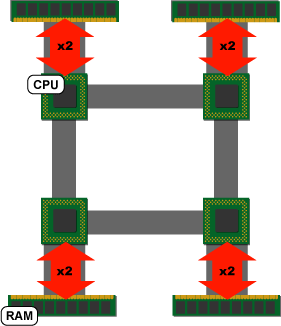
\includegraphics[height=5cm]{quad-opteron-numa.png}
  \end{center}
  \creditto{arstechnica.com}
  \uncover<+->{}
  \uncover<+->{
    \begin{tikzpicture} [overlay]
      \node [above left=1cm of current page.south east,draw,drop shadow,fill=white,
       inner sep=5mm,thick]
        {
          ``NUMA''
        } ;
    \end{tikzpicture}
  }
\end{frame}
% -----------------------------------------------------------------------------
\begin{frame}{NUMA demo}
  \begin{center}
  \Huge Contention/throughput demo
  \end{center}
\end{frame}
% -----------------------------------------------------------------------------
\begin{frame}[fragile]{NUMA results}
  \texttt{`crunchy3'} at Courant

  \medskip
  \begin{lstlisting}
    num cpus: 32
    numa available: 0
    numa node 0 10001000100010000000000000000000 - 15.9904 GiB
    numa node 1 00000000000000001000100010001000 - 16 GiB
    numa node 2 00010001000100010000000000000000 - 16 GiB
    numa node 3 00000000000000000001000100010001 - 16 GiB
    numa node 4 00100010001000100000000000000000 - 16 GiB
    numa node 5 00000000000000000010001000100010 - 16 GiB
    numa node 6 01000100010001000000000000000000 - 16 GiB
    numa node 7 00000000000000000100010001000100 - 16 GiB
  \end{lstlisting}
\end{frame}
% -----------------------------------------------------------------------------
\begin{frame}[fragile]{NUMA results}
  \texttt{`crunchy3'} at Courant

  \medskip
  \begin{lstlisting}
    sequential core 0 -> core 0 : BW 4189.87 MB/s
    sequential core 1 -> core 0 : BW 2409.1 MB/s
    sequential core 2 -> core 0 : BW 2495.61 MB/s
    sequential core 3 -> core 0 : BW 2474.62 MB/s
    sequential core 4 -> core 0 : BW 4244.45 MB/s
    sequential core 5 -> core 0 : BW 2378.34 MB/s
    ....
    sequential core 29 -> core 0 : BW 2048.68 MB/s
    sequential core 30 -> core 0 : BW 2087.6 MB/s
    sequential core 31 -> core 0 : BW 2014.68 MB/s
  \end{lstlisting}
\end{frame}
% -----------------------------------------------------------------------------
\begin{frame}[fragile]{NUMA results}
  \texttt{`crunchy3'} at Courant

  \medskip
  \begin{lstlisting}
    all-contention core 0 -> core 0 : BW 1081.85 MB/s
    all-contention core 1 -> core 0 : BW 299.177 MB/s
    all-contention core 2 -> core 0 : BW 298.853 MB/s
    all-contention core 3 -> core 0 : BW 263.735 MB/s
    all-contention core 4 -> core 0 : BW 1081.93 MB/s
    all-contention core 5 -> core 0 : BW 299.177 MB/s
    ....
    all-contention core 27 -> core 0 : BW 202.49 MB/s
    all-contention core 28 -> core 0 : BW 434.295 MB/s
    all-contention core 29 -> core 0 : BW 233.309 MB/s
    all-contention core 30 -> core 0 : BW 233.169 MB/s
    all-contention core 31 -> core 0 : BW 202.526 MB/s
  \end{lstlisting}
\end{frame}
% -----------------------------------------------------------------------------
\begin{frame}[fragile]{NUMA results}
  \texttt{`crunchy3'} at Courant

  \medskip
  \begin{lstlisting}
    two-contention core 0 -> core 0 : BW 3306.11 MB/s
    two-contention core 1 -> core 0 : BW 2199.7 MB/s

    two-contention core 0 -> core 0 : BW 3257.56 MB/s
    two-contention core 19 -> core 0 : BW 1885.03 MB/s
  \end{lstlisting}
\end{frame}
% -----------------------------------------------------------------------------
\begin{frame}{NUMA? Do I need to care?}
  Large multi-core machines \emph{are} NUMA.

  \bigskip
  Also: Easy, can use OpenMP $\rightarrow$ popular

  \bigskip
  What happens if you ignore NUMA?
  \begin{itemize}
    \item What happens at \texttt{malloc}?
    \item What happens at `first touch'?
    \item What happens if you don't pin-to-core?
  \end{itemize}
\end{frame}
% -----------------------------------------------------------------------------
\subsection{Non-memory-related}
% -----------------------------------------------------------------------------
\begin{frame}{Recap: superscalar architecture}
  \begin{center}
  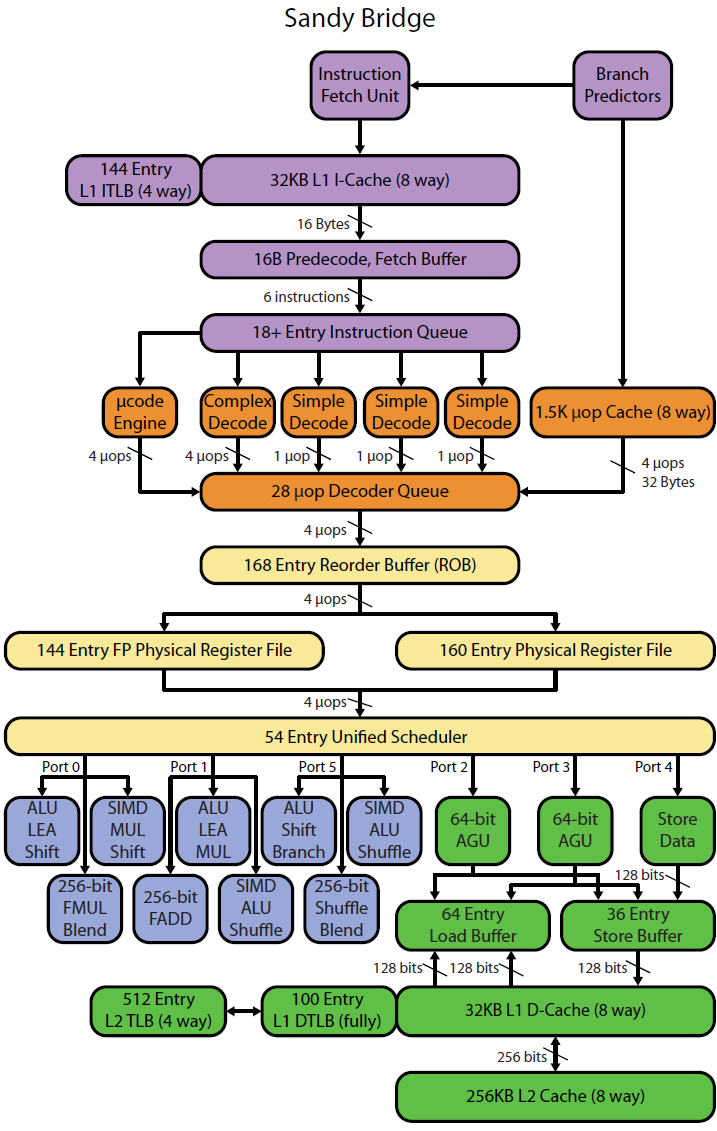
\includegraphics[height=0.85\textheight]{sandy-bridge-pipeline.png}
  \end{center}

  \creditto{David Kanter / Realworldtech.com}
  \uncover<2>{
    \begin{tikzpicture} [overlay]
      \node [above right=1cm of current page.south east,
        draw,drop shadow,fill=white,xshift=-0.5cm,yshift=-0.5cm,
        text width=0.6\textwidth, inner sep=3mm,thick]
        {
          What if some units are unused?
        } ;
    \end{tikzpicture}
  }
\end{frame}
% -----------------------------------------------------------------------------
\begin{frame}{SMT/``Hyperthreading''}

  \begin{center}
    \begin{tikzpicture}
      \node [draw,thick,fill=red!30,minimum width=4cm,minimum height=1cm]
        (fe) { Processor front end };

      \foreach \i/\ofs in {1/-1.5, 2/-0.75, 3/0, 4/0.75,5/1.5}
      {
        \ifthenelse{\i < 4}
        { \def\itemcolor{green!30} }
        {
          \ifthenelse{\overlaynumber = 1}
          { \def\itemcolor{gray!20} }
          { \def\itemcolor{blue!30} }
          { }
        }

        \node [draw,thick,fill=\itemcolor,rotate=270,below=2cm of
        fe,anchor=center,yshift=\ofs cm]
          (exec\i) { Exec. Unit \i };
        \draw [thick,->] (fe) -- (exec\i.west);
      }

      \uncover<1>{
        \node[single arrow,draw,thick,shape border
        rotate=270,fill=green!30,above=0cm of fe]
        {
          Program
        };
      }
      \uncover<2->{
        \node[single arrow,draw,thick,shape border
        rotate=270,fill=green!30,above=0cm of fe,xshift=-0.5cm]
        {
          Thread 1
        };
        \node[single arrow,draw,thick,shape border
        rotate=270,fill=blue!30,above=0cm of fe,xshift=0.5cm]
        {
          Thread 2
        };
      }
    \end{tikzpicture}
  \end{center}

  \uncover<+>{}
  \uncover<+>{}
  \uncover<+->{
    \begin{tikzpicture} [overlay]
      \node [above left=1cm of current page.south east,
        draw,thick,drop shadow,fill=white, inner sep=3mm,
        text width=0.6\textwidth]
        {
          Potential issues?
          \only<+->{
            \begin{itemize}
              \item $n\times$ the cache demand!
              \item Power?
            \end{itemize}
            $\rightarrow$ Some people just turn it off and manage
            their own ILP.
          }
        } ;
    \end{tikzpicture}
  }
\end{frame}
% -----------------------------------------------------------------------------
\begin{frame}{Locks}
  \begin{center}
  \Large Locks are not slow

  \bigskip
  Lock \emph{contention} is slow

  \end{center}
  \uncover<+>{}
  \uncover<+>{
    \begin{tikzpicture} [overlay]
      \node [above left=1cm of current page.south east,
      draw,thick,drop shadow,fill=white, inner sep=3mm]
        {
          Demo, also $\rightarrow$ HW2
        } ;
    \end{tikzpicture}
  }
\end{frame}


% }}}
% -----------------------------------------------------------------------------
\section{GPU performance}
% -----------------------------------------------------------------------------
% {{{
% -----------------------------------------------------------------------------
\subsection{Less control, more data}
% -----------------------------------------------------------------------------
\newcommand{\kayvoncredit}{
  \begin{tikzpicture}[overlay]
    \node [xshift=1cm,yshift=0.5cm]
      at (current page.south west)
      [font=\scriptsize,fill=gray!30,anchor=south west,opacity=0.5]
      {Credit: Kayvon Fatahalian (Stanford) };
  \end{tikzpicture}
}
\newcommand{\kayvonframe}[5]{

  \begin{frame}{#1}
    #4
    \begin{center}
    \includegraphics[viewport=#3,clip=true,page=#2,height=0.7\textheight]{kayvon-gpuarch.pdf}
    \end{center}
    \kayvoncredit
    #5
  \end{frame}
}
\kayvonframe{Gratuitous Amounts of Parallelism!}{24}{5in 1.45in 10in 6.75in }{}{
  \uncover<2->{
    \begin{tikzpicture} [overlay]
      \node [below right=1.75cm of current page.north west, draw,drop shadow,fill=white,
      text width=0.8\textwidth, inner sep=2.5mm,thick]
        {
          Example:

          \medskip
          128 instruction streams in parallel

          16 independent groups of 8 synchronized streams
        } ;
    \end{tikzpicture}
  }
  \uncover<3>{
    \begin{tikzpicture} [overlay]
      \node [above left=1cm of current page.south east, draw,drop shadow,fill=white,
      text width=0.6\textwidth, inner xsep=0.5cm,inner ysep=0.5cm,thick]
        {
          Great if everybody in a group does the same thing.

          \medskip
          But what if not?

          \medskip
          What leads to divergent instruction streams?
        } ;
    \end{tikzpicture}
  }
}
\kayvonframe{Branches}{26}{0.85in 0.9in 10.5in 6.8in }{}{}
\kayvonframe{Branches}{27}{0.85in 0.9in 10.5in 6.8in }{}{}
\kayvonframe{Branches}{28}{0.85in 0.9in 10.5in 6.8in }{}{}
\kayvonframe{Branches}{29}{0.85in 0.9in 10.5in 6.8in }{}{}
% -----------------------------------------------------------------------------
\begin{frame}{GPUs vs Branching}
  \begin{center}
  \Huge Branch demo time
  \end{center}
\end{frame}
% -----------------------------------------------------------------------------
\subsection{GPUs and Latency}
% -----------------------------------------------------------------------------
\begin{frame}{GPUs vs Latency}
  \begin{columns}
    \column{0.6\textwidth}
      \begin{block}{Problem}
        Memory still has very high latency\dots

        \dots as do many other things\dots

        \dots but we've removed most of the hardware that helps us
        deal with that.

      \end{block}
      \medskip
      We've removed
      \begin{itemize}
      \item caches
      \item branch prediction
      \item out-of-order execution
      \end{itemize}

      So what now?
    \column{0.4\textwidth}
      \includegraphics[width=\textwidth]{memory.png}
  \end{columns}
  \uncover<2->{
    \begin{tikzpicture} [overlay]
      \node [below right=1cm of current page.north west, draw,drop shadow,fill=white,
      text width=0.6\textwidth, inner sep=5mm,thick]
      {
        \only<2-3>{\includegraphics[viewport=6.25in 1in 10.25in 4.75in,clip=true,page=33,width=\textwidth]{kayvon-gpuarch.pdf}}%
        \only<4>{\includegraphics[viewport=6.25in 1in 10.25in 4.75in,clip=true,page=34,width=\textwidth]{kayvon-gpuarch.pdf}}%
      };
    \end{tikzpicture}
  }
  \uncover<3->{
    \begin{tikzpicture} [overlay]
      \node [above left=1cm of current page.south east, draw,drop shadow,fill=white,
      text width=0.4\textwidth, inner sep=5mm,thick]
      {
        \textbf{Idea \#3}

        \medskip
        \begin{tabular}{rl}
        & Even more parallelism \\ + &Some extra memory \\ \hline = &A solution!
        \end{tabular}

      };
    \end{tikzpicture}
  }
\end{frame}

\kayvonframe{Hiding Memory Latency}{33}{0.65in 0.85in 10.4in 6.8in }{}{}
\kayvonframe{Hiding Memory Latency}{34}{0.65in 0.85in 10.4in 6.8in }{}{}
\kayvonframe{Hiding Memory Latency}{35}{0.65in 0.85in 10.4in 6.8in }{}{}
\kayvonframe{Hiding Memory Latency}{36}{0.65in 0.85in 10.4in 6.8in }{}{}
\kayvonframe{Hiding Memory Latency}{37}{0.65in 0.85in 10.4in 6.8in }{}{}
\kayvonframe{Hiding Memory Latency}{38}{0.65in 0.85in 10.4in 6.8in }{}{}

% -----------------------------------------------------------------------------
\begin{frame}{Architecture}
  \begin{center}
  \Huge GPUs and latency demo
  \end{center}
\end{frame}
% -----------------------------------------------------------------------------
\subsection{Understanding GPUs}
% -----------------------------------------------------------------------------
\begin{frame}{Comparing architectures}
  \begin{tabular}{l|cccc|l}
    & GF100 & GF104 & GK104 & GCN & Units\\
    \hline
    \# Warps/Wavefronts & 48 & 48 & 64 & 40 \\
    Warp Size & 32 & 32 & 32 & 64 & W.Item \\
    \hline
    SP FLOP/clock & 64 & 96 & 384 & 128 \\
    Clock & 700 & 650 & 823 & 925 & MHz \\
    \hline
    Reg File & 128 & 128 & 256 & 256 & kiB \\
    Lmem & 64  & 64 & 64 & 64 & kiB \\
    Lmem BW & 64  & 64 & 128 & 128 & B/clock \\
    \hline
  \end{tabular}
  \creditto{David Kanter / Realworldtech.com}
\end{frame}
% -----------------------------------------------------------------------------
\begin{frame}{Architecture}
  \begin{center}
  \Huge Architecture by the numbers demo
  \end{center}
\end{frame}
% -----------------------------------------------------------------------------
\begin{frame}{Architecture}
  \begin{center}
  \Huge Occupancy calculator
  \end{center}
\end{frame}
% -----------------------------------------------------------------------------
\subsection{GPUs and Memory}
% -----------------------------------------------------------------------------
\input{parallel-memories}
\input{cl-gmem-access}
% -----------------------------------------------------------------------------
\begin{frame}{GPU Global Memory}
  \begin{center}
  \Huge GPU global access patterns demo
  \end{center}
\end{frame}
% -----------------------------------------------------------------------------
\input{cl-lmem-access}
% -----------------------------------------------------------------------------
\begin{frame}{GPU local Memory}
  \begin{center}
  \Huge GPU local access patterns demo
  \end{center}
\end{frame}
% -----------------------------------------------------------------------------
\begin{frame}{Entertainment: GPU Memory Zoo}

  \uncover<+->{
    \begin{tabular}{p{5em}cccp{2.8cm}}
    \hline
    \textbf{Type} & \textbf{Per} & \textbf{Access} & \textbf{Latency} \\
    \hline
    \textbf<2->{private} & work item & R/W & 1 or 1000 \\
    \textbf<2->{local} & group & R/W & 2 \\
    \textbf<2->{global} & grid & R/W & 1000 & Cached?\\
    \texttt{constant} & grid & R/O & 1-1000 & Cached \\
    image$n$d\_t & grid & R(/W) & 1000 & Spatially cached\\
    \hline
    \end{tabular}
  }

\end{frame}
% -----------------------------------------------------------------------------
\subsection{Summary}
% -----------------------------------------------------------------------------
\begin{frame}{GPU performance summary}
\end{frame}

% }}}

% {{{

% TODO:
% Global mem performance:
% 
% - Alignment
% - Strides
% 
% Local mem
% - Banking

% case study: optimize mat-mat

% }}}
\questionframe{}
\imagecreditslide

\end{document}
% vim: foldmethod=marker


